% gm-13-conics.tex

\documentclass[xcolor=dvipsnames]{beamer}

\usepackage{cancel}
\renewcommand{\CancelColor}{\color{red}}
\usepackage{graphicx}
\usepackage{wrapfig}
\usepackage{colortbl}
\usepackage{color}
\usepackage{alltt}
\renewcommand*{\thefootnote}{\fnsymbol{footnote}}
\definecolor{myblue}{rgb}{0.8,0.85,1}

\mode<presentation>
{
  \usetheme{Warsaw}
  \setbeamercovered{transparent}
}
% \usecolortheme[named=OliveGreen]{structure}
\setbeamertemplate{navigation symbols}{} 
\setbeamertemplate{blocks}[rounded][shadow=true] 

% this is for overlaying math symbols, see https://tex.stackexchange.com/questions/12895/overlay-symbol-with-another
\def\qeq{\mathrel{%
    \mathchoice{\QEQ}{\QEQ}{\scriptsize\QEQ}{\tiny\QEQ}%
}}
\def\QEQ{{%
    \setbox0\hbox{$\longrightarrow$}%
    \rlap{\hbox to \wd0{\hss/\hss}}\box0
  }}

\newcounter{expls}
\setcounter{expls}{0}
\newcommand{\beispiel}[1]{\refstepcounter{expls}\textbf{Example \arabic{expls}: #1.}}

\newcounter{exercise}
\setcounter{exercise}{0}
\newcommand{\ubung}[0]{\refstepcounter{exercise}\textbf{Exercise \arabic{exercise}: }}

\newif\ifBCITCourse
\BCITCoursetrue
% \BCITCoursefalse
\newif\ifWhichCourse
\WhichCoursetrue
\WhichCoursefalse
\ifBCITCourse
\ifWhichCourse
\newcommand{\CourseName}{Technical Mathematics for Food Technology}
\newcommand{\CourseNumber}{MATH 1441}
\newcommand{\CourseInst}{BCIT}
\else
\newcommand{\CourseName}{Technical Mathematics for Geomatics}
\newcommand{\CourseNumber}{MATH 1511}
\newcommand{\CourseInst}{BCIT}
\fi
\else
\newcommand{\CourseName}{Philosophy and Literature}
\newcommand{\CourseNumber}{PHIL 375}
\newcommand{\CourseInst}{UBC}
\fi

\title{Conics}
\subtitle{{\CourseNumber}, BCIT}

\author{\CourseName}

\date{October 30, 2017}

\begin{document}

\begin{frame}
  \titlepage
\end{frame}

\begin{frame}
  \frametitle{Curves}
Equations have solution sets. These solution sets are subsets of
spaces like the number line (one variable), the plane (two variables),
or three-dimensional space (three variables). When there are two
variables, the solution set may describe a curve. A curve is a
one-dimensional space inside a higher-dimensional space, for example
the plane. The most simple example is the circle. Consider the
equation
  \begin{figure}[h]
    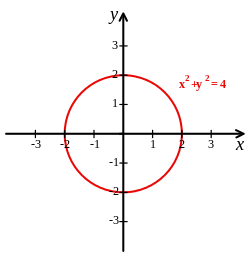
\includegraphics[scale=.5]{./circle.png}
  \end{figure}
\end{frame}

\begin{frame}
  \frametitle{Polynomials}
The following expression is called a polynomial.
\begin{equation}
  \label{eq:eeheemei}
f(x)=a_{n}x^{n}+a_{n-1}x^{n-1}+\ldots{}+a_{2}x^{2}+a_{1}x+a_{0}
\end{equation}
For example, $f(x)=x^{3}+5x^{2}+7x+2$. $n\geq{}0$ is a natural number
called the \alert{degree of the polynomial}, and the $a_{i}$ are real
numbers called \alert{coefficients}. Here is what a curve described by
a polynomial with degree $3$ looks like.
  \begin{figure}[h]
    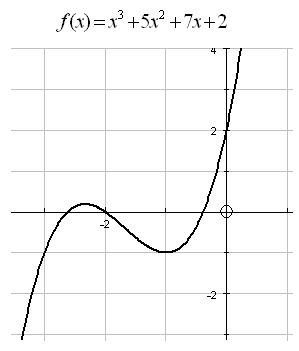
\includegraphics[scale=.35]{./third.png}
  \end{figure}
\end{frame}

\begin{frame}
  \frametitle{Equations and Curves}
  Curves in the plane may correspond to equations with two variables,
  as in the example with the circle. Sometimes, we push everything in
  the equation to the LHS (left-hand side) and leave $0$ on the RHS
  (right-hand side). For the circle,
\begin{equation}
  \label{eq:fuazegho}
x^{2}+y^{2}-4=0
\end{equation}
and for the polynomial in the last slide,
\begin{equation}
  \label{eq:iivoixah}
x^{3}+5x^{2}+7x+2-y=0
\end{equation}
\end{frame}

\begin{frame}
  \frametitle{Conics I}
  It turns out that all curves that correspond to polynomials of
  degree 2 or less in two-dimensional space are conic sections or
  \alert{conics}. Equations such as
\begin{equation}
  \label{eq:aipheiyu}
Ax^{2}+Bxy+Cy^{2}+Dx+Ey+F=0
\end{equation}
with $A,B,C,D,E,F$ being real numbers (with $|A|+|B|+|C|\neq{}0$)
correspond to curves that can be thought of as intersections of the
plane with a \alert{parabola}, an \alert{ellipse}, or a
\alert{hyperbola}.
  \begin{figure}[h]
    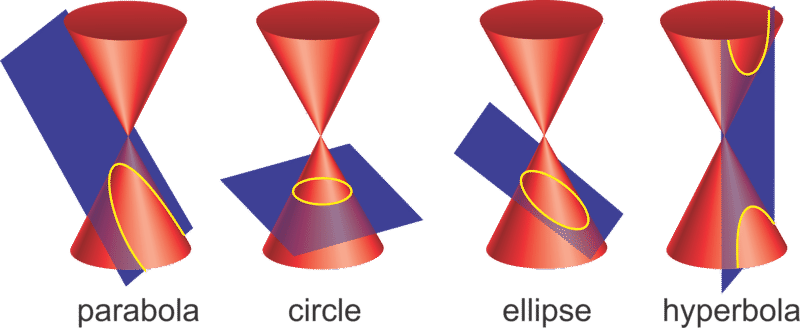
\includegraphics[scale=.35]{./conics1.png}
  \end{figure}
\end{frame}

\begin{frame}
  \frametitle{Conics II}
Circles are just special cases of ellipses. Is the polynomial curve
with degree 3 from a couple of slides ago a conic? Why (not)?
  \begin{figure}[h]
    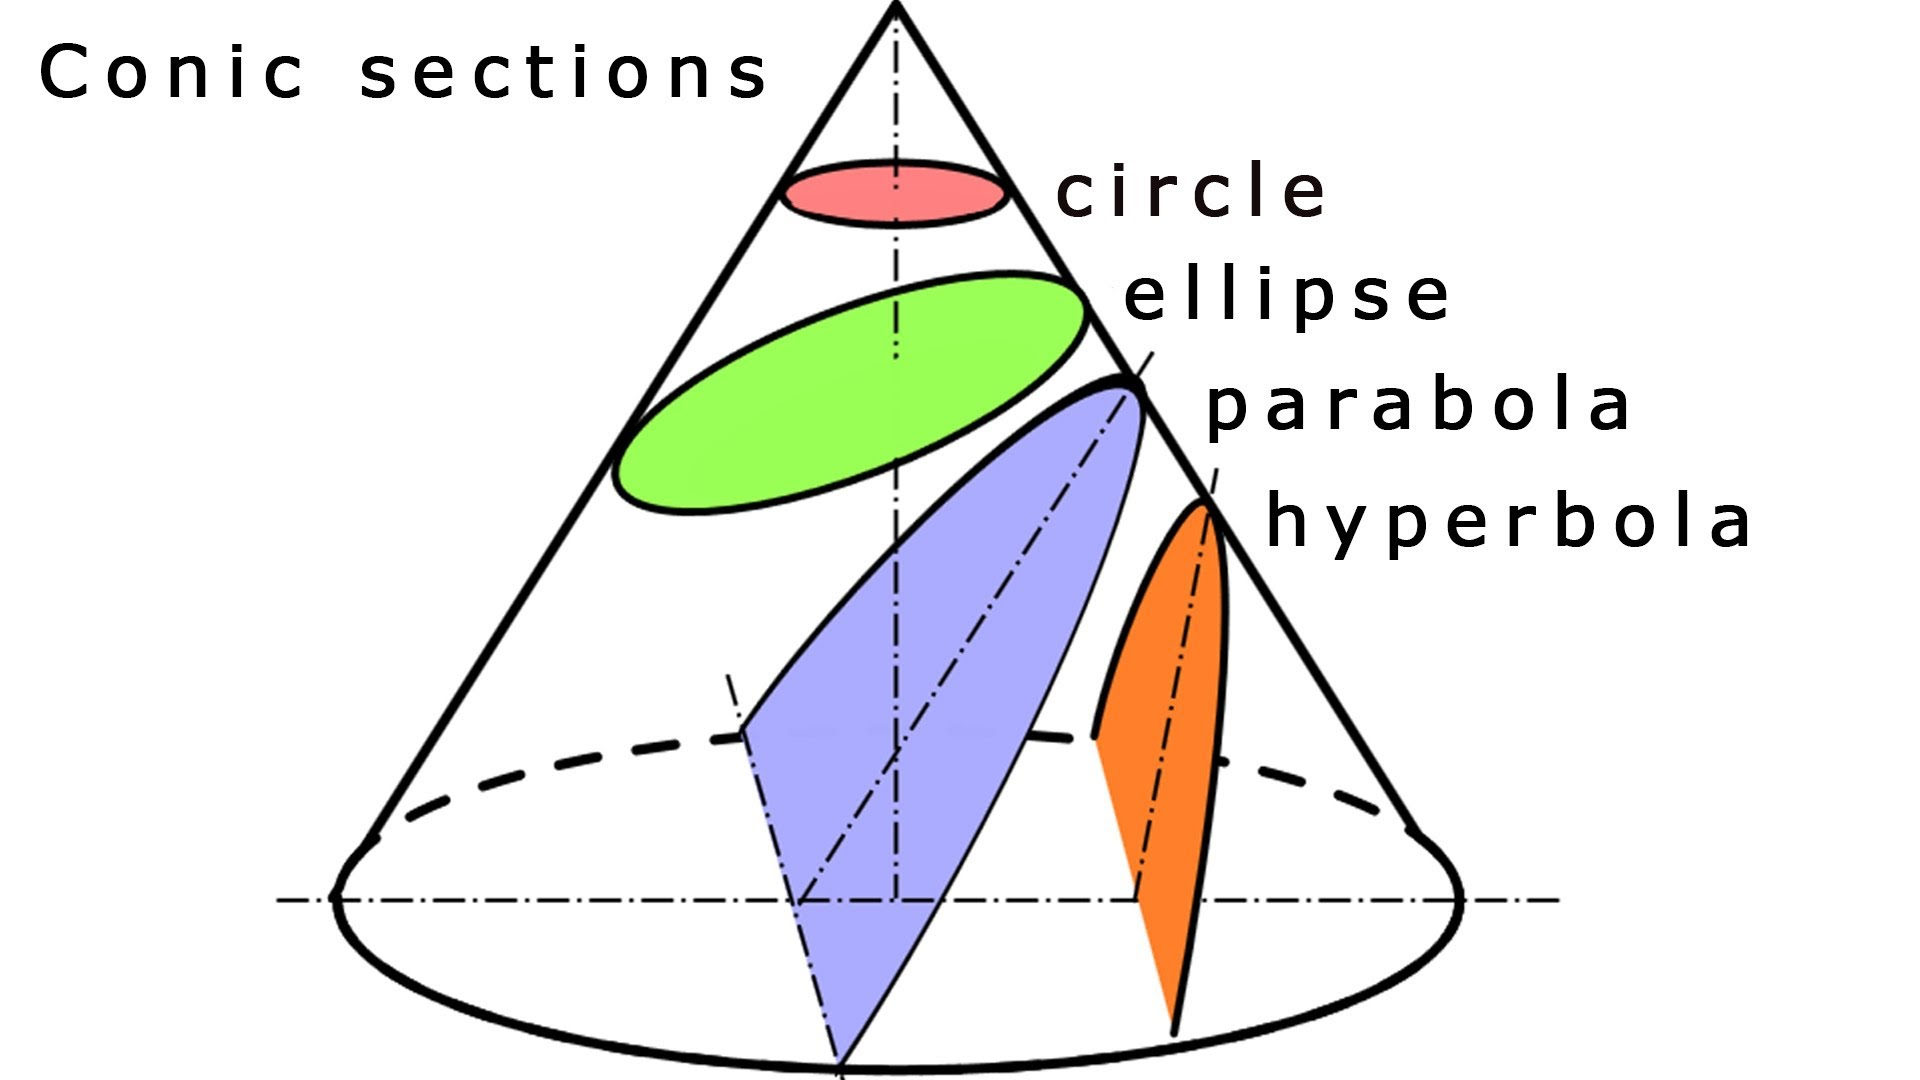
\includegraphics[scale=.17]{./conics2.jpg}
  \end{figure}
\end{frame}

\begin{frame}
  \frametitle{Conics III}
  If (for now $B$ is always zero in order to avoid conics whose
  symmetries do not line up with the coordinate system)
\begin{equation}
  \label{eq:adailaek}
Ax^{2}+Bxy+Cy^{2}+Dx+Ey+F=0
\end{equation}
is the equation of the conic section, then $B^{2}-4AC$ is the
\alert{discriminant} of the equation. 
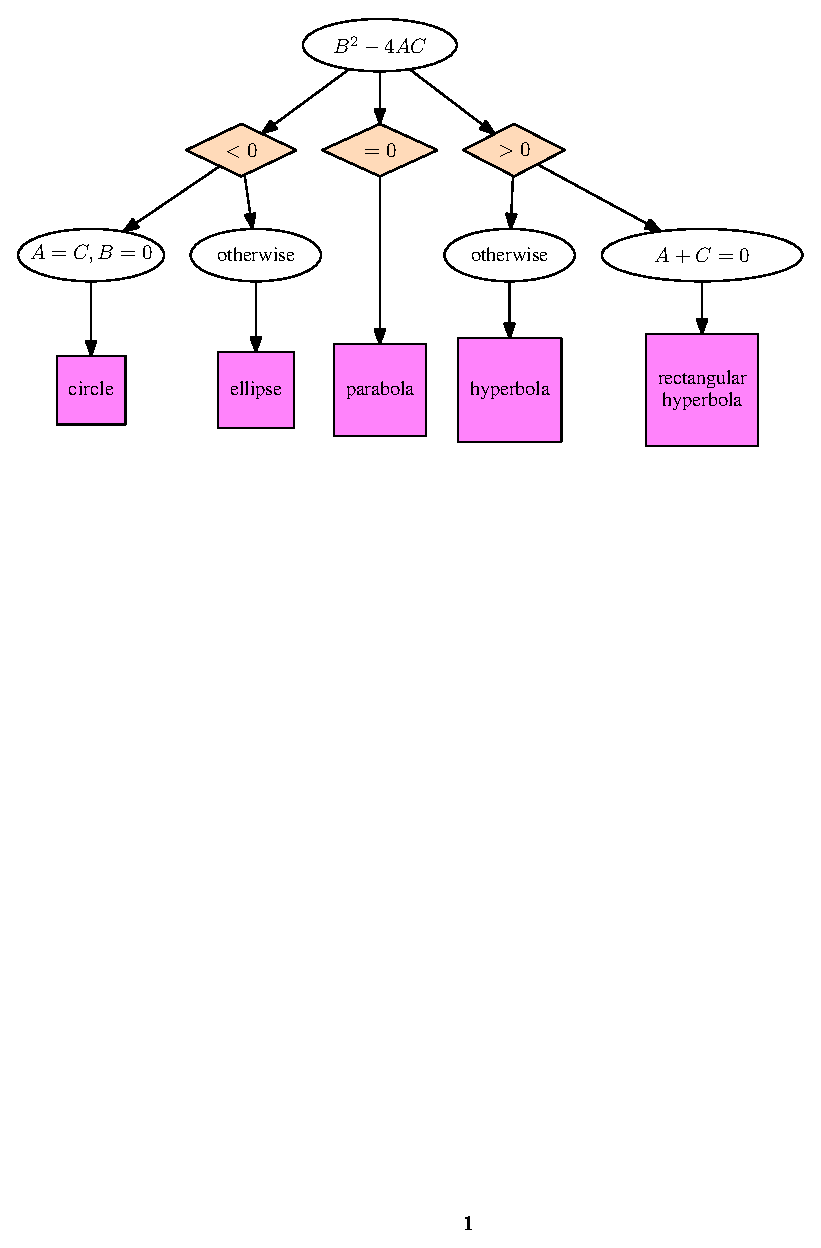
\includegraphics[scale=.65]{conicdiscriminant.eps}
\end{frame}

\begin{frame}
  \frametitle{Conics Exercises}
Classify the following equations according to the type of conic each represents.
\begin{enumerate}
\item<1-> $3x^{2}+3y^{2}-6x+9y-14=0$
\item<2-> $6x^{2}+12x-y+15=0$
\item<3-> $x^{2}+2y^{2}+4x+2y-27=0$
\item<4-> $x^{2}-y^{2}+3x-2y-43=0$
\end{enumerate}
\end{frame}

\begin{frame}
  \frametitle{Parabolas}
Here is one form of a parabola, which tells us where the
vertex is. The vertex is the point where the line of symmetry
intersects with the parabola.
\begin{equation}
  \label{eq:aizienah}
y=a(x-p)^{2}+q\mbox{ or }x=a(y-q)^{2}+p
\end{equation}
$a\neq{}0,p,q$ are real numbers. The vertex is at $(p,q)$.
\begin{itemize}
\item If $a>0$ and $y$ is not squared, then the parabola opens upward. The parabola is \alert{convex}.
\item If $a<0$ and $y$ is not squared, then the parabola opens downward. The parabola is \alert{concave}.
\item If $a>0$ and $x$ is not squared, then the parabola opens to the right. 
\item If $a<0$ and $x$ is not squared, then the parabola opens to the left. 
\end{itemize}
Exercise: determine whether the functions $f(x)=e^{x}$ and
$g(x)=\ln{}x$ are convex or concave.
\end{frame}

\begin{frame}
  \frametitle{Vertex, Focus, Directrix}
  Besides a \alert{vertex}, a parabola also has a \alert{focus} and a
  \alert{directrix} (two out of these three uniquely determine a
  parabola). You may learn later how to calculate them given the
  equation of the parabola; or to determine the equation for the
  parabola, given the focus and the directrix. All points on a
  parabola are equidistant (equally far away) from the directrix and
  the focus.
  \begin{figure}[h]
    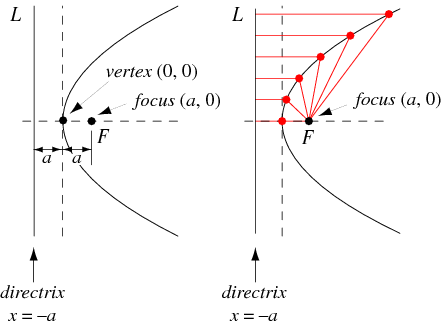
\includegraphics[scale=.45]{./parabola.png}
  \end{figure}
\end{frame}

\begin{frame}
  \frametitle{Parabola Exercises}
Consider the following curve.
\begin{equation}
  \label{eq:eicaemae}
  2y^{2}-\frac{1}{2}x-12y+19=0
\end{equation}
Use the discriminant to show that the curve is a parabola. Calculate
the position of the vertex and determine whether the parabola opens
upward, downward, to the right, or to the left. 

\medskip

Try again with the following equation.
\begin{equation}
  \label{eq:xohsheco}
-63x^{2}+84x+315y=253
\end{equation}
\end{frame}

\begin{frame}
  \frametitle{Parabola Exercise Solution}
  \begin{figure}[h]
    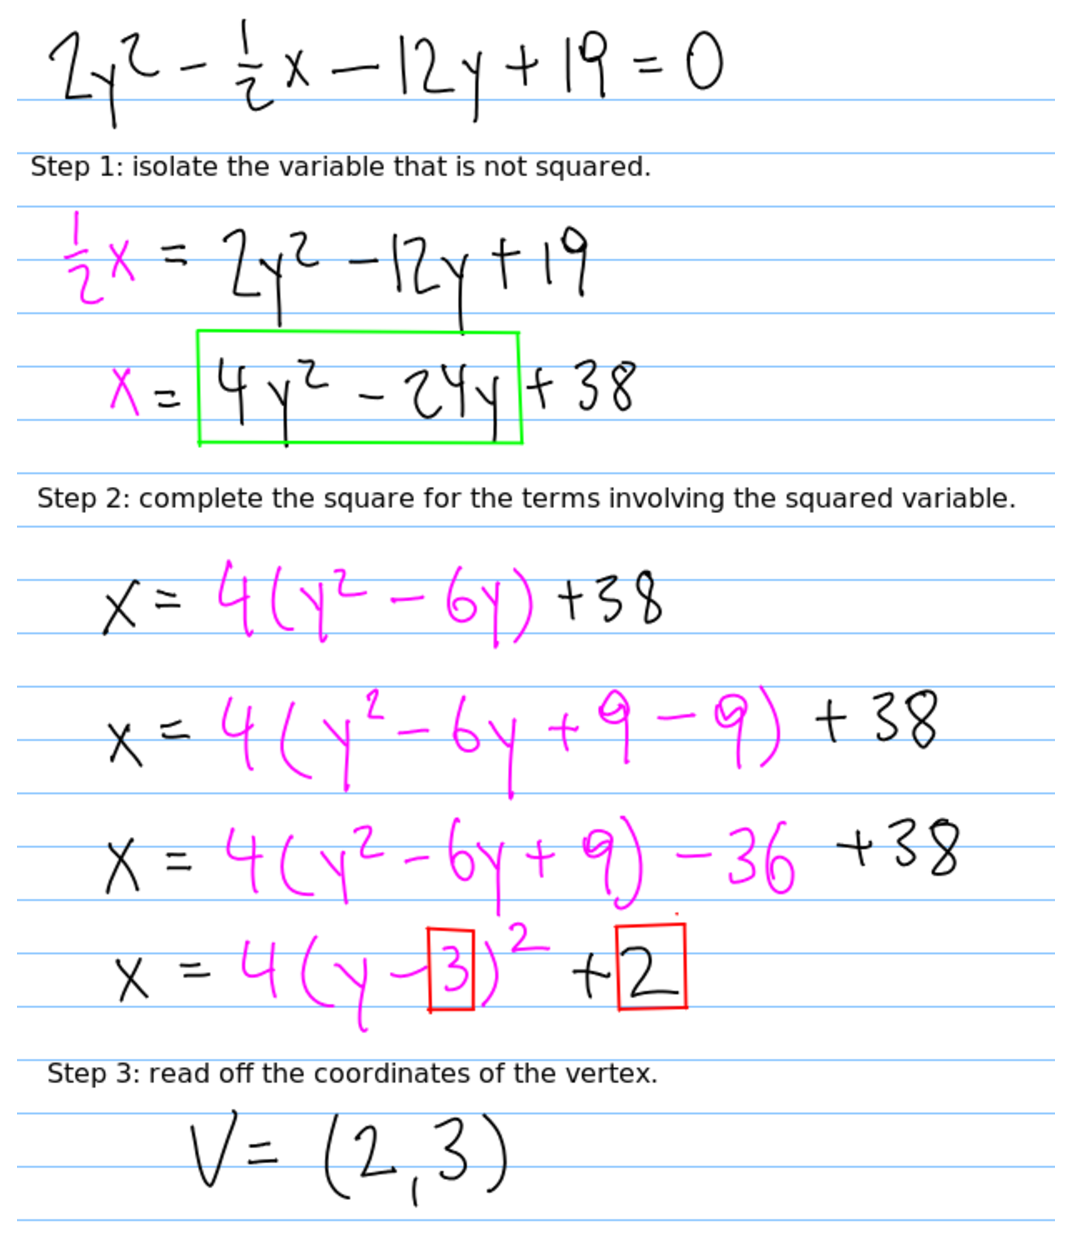
\includegraphics[scale=.4]{./parabola.eps}
  \end{figure}
\end{frame}

\begin{frame}
  \frametitle{Parabola Exercise Solutions}
\begin{equation}
  \label{eq:zeiquahn}
  2y^{2}-\frac{1}{2}x-12y+19\longrightarrow{}x=4(y-3)^{2}+2
\end{equation}
The vertex is $V=(2,3)$.

\medskip

\begin{equation}
  \label{eq:kaitoohe}
-63x^{2}+84x+315y=253\longrightarrow{}y=\frac{1}{5}\left(x-\frac{2}{3}\right)^{2}+\frac{5}{7}
\end{equation}
The vertex is $V=\left(\frac{2}{3},\frac{5}{7}\right)$.
\end{frame}

\begin{frame}
  \frametitle{Circle}
  Here is one form of a circle, which tells us where the
  \alert{centre} of the circle and the \alert{radius} are.
\begin{equation}
  \label{eq:ainguxuf}
(x-p)^{2}+(y-q)^{2}=r^{2}
\end{equation}

Find centre and radius for the following two circle
equations. 
\begin{equation}
  \label{eq:kahdaixi}
x^{2}+y^{2}-4x-21=0
\end{equation}
\begin{equation}
  \label{eq:adeongie}
x^{2}+y^{2}-4x-6y-3=0
\end{equation}
Now, find the equation of the circle for which the centre is $M=(4,-2)$
and the radius is $r=10$.
\end{frame}

\begin{frame}
  \frametitle{Ellipse I}
There is a lot going on when we consider an ellipse. Consider the
following diagram.
  \begin{figure}[h]
    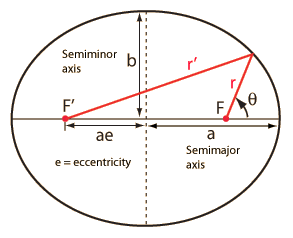
\includegraphics[scale=.65]{./elliporb.png}
  \end{figure}
\end{frame}

\begin{frame}
  \frametitle{Ellipse II}
  One way to define an ellipse is to say that for all points $P$ on an
  ellipse, the distance of $P$ from the two points of \alert{focus}
  sum to a constant. This constant is $2a$, two times the
  \alert{semimajor axis}.

Here is how we will define an ellipse. Points on an ellipse fulfill
the equation
\begin{equation}
  \label{eq:aiyohboo}
  \frac{(x-p)^{2}}{a^{2}}+\frac{(y-q)^{2}}{b^{2}}=1
\end{equation}
The \alert{centre of the ellipse} is at $M=(p,q)$. $a$ is the length
of the semimajor axis, $b$ is the length of the \alert{semiminor
  axis}.
\end{frame}

\begin{frame}
  \frametitle{Ellipse Exercises}
Determine centre and dimensions of the following ellipse,
\begin{equation}
  \label{eq:veatoiyu}
x^{2}+2y^{2}=2  
\end{equation}
Do the same for the following ellipse,
\begin{equation}
  \label{eq:kohvoigh}
9x^{2}-18x+4y^{2}+40y=-73
\end{equation}
\end{frame}

\begin{frame}
  \frametitle{Hyperbola I}
  A hyperbola, just like an ellipse, has two points of \alert{focus}.
  The hyperbola is the set of points for which the difference of the
  distance to the two foci is constant. This difference, again
  analogous to an ellipse, is $2a$, which is also the distance between
  the two \alert{vertices} of the hyperbola. 
  \begin{figure}[h]
    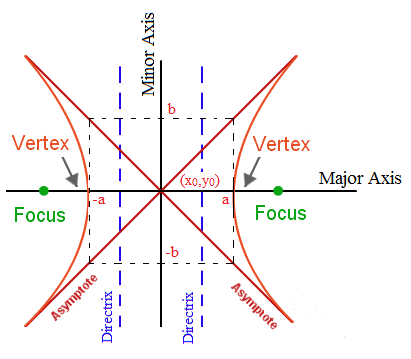
\includegraphics[scale=.6]{./hyperbola.png}
  \end{figure}
\end{frame}

\begin{frame}
  \frametitle{Hyperbola II}
  Hyperbolas have two branches which approach lines called
  \alert{asymptotes}. There is also a \alert{major axis} and a
  \alert{minor axis}. The major axis is sometimes called the
  \alert{transverse axis}. If the two asymptotes are perpendicular to
  each other, the hyperbola is a \alert{rectangular hyperbola}. The
  function $f(x)=1/x$ is the graph of a rectangular hyperbola.
\end{frame}

\begin{frame}
  \frametitle{Hyperbola III}
  If the transverse axis is horizontal, one form of an equation for a
  hyperbola identifying the centre $M$ is
\begin{equation}
  \label{eq:leiweidi}
\frac{(x-p)^{2}}{a^{2}}-\frac{(y-q)^{2}}{b^{2}}=1
\end{equation}
  If the transverse axis is vertical, one form of an equation for a
  hyperbola identifying the centre $M$ is
\begin{equation}
  \label{eq:aewailei}
\frac{(y-q)^{2}}{a^{2}}-\frac{(x-p)^{2}}{b^{2}}=1
\end{equation}
\end{frame}

\begin{frame}
  \frametitle{Hyperbola Exercises}
  Find the centre, vertices, foci, eccentricity, and asymptotes of the
  hyperbola with the given equation, and sketch,
\begin{equation}
  \label{eq:eezeisud}
\frac{y^{2}}{25}-\frac{x^{2}}{144}=1
\end{equation}
Give the center, vertices, foci, and asymptotes for the hyperbola
with equation,
\begin{equation}
  \label{eq:utheikuv}
\frac{(x+3)^{2}}{16}-\frac{(y-2)^{2}}{9}=1
\end{equation}
Find the center, vertices, and asymptotes of the hyperbola with
equation,
\begin{equation}
  \label{eq:beizooph}
4x^{2}-5y^{2}+40x-30y-45=0
\end{equation}
\end{frame}

\begin{frame}
  \frametitle{Hyperbola Exercise Solution}
\begin{equation}
  \label{eq:ieyuipoo}
\frac{(x+3)^{2}}{16}-\frac{(y-2)^{2}}{9}=1
\end{equation}
The centre is $M=(-3,2)$. The dimensions are $a=4,b=3$. Because the
coefficient for $x^{2}$ is positive and the coefficient for $y^{2}$ is
negative, the transverse axis is horizontal. Considering that
$P_{1}=(1,5)$ and $M$ are on the upward-sloping asymptote $A_{1}$, the
equation for $A_{1}$ is 
\begin{equation}
  \label{eq:maighere}
y=\frac{3}{4}x+\frac{17}{4}
\end{equation}
Considering that
$P_{2}=(1,-1)$ and $M$ are on the downward-sloping asymptote $A_{2}$, the equation for $A_{2}$ is 
\begin{equation}
  \label{eq:eeleeyae}
y=-\frac{3}{4}x-\frac{1}{4}
\end{equation}
\end{frame}

\begin{frame}
  \frametitle{Hyperbola Exercise Solution Diagram}
  \begin{figure}[h]
    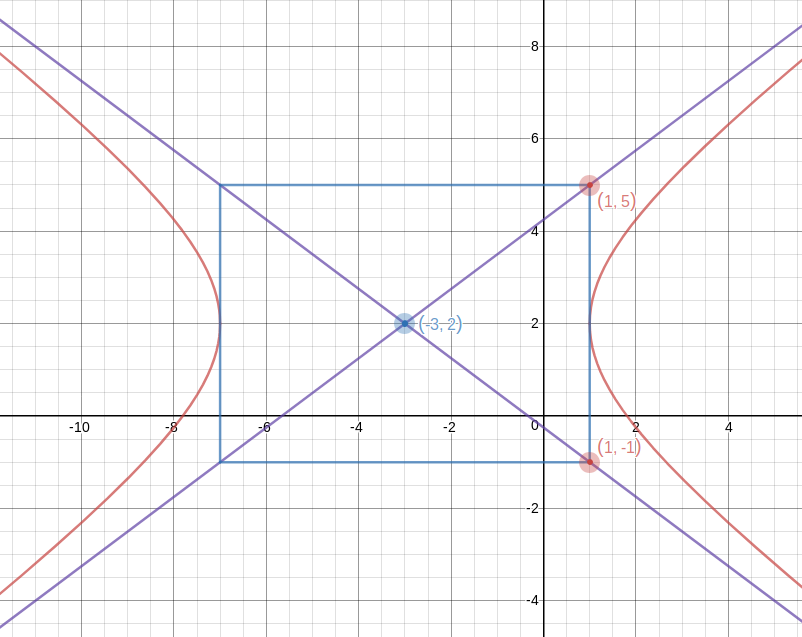
\includegraphics[scale=.5]{./hyperbola3.png}
  \end{figure}
\end{frame}

\begin{frame}
  \frametitle{Eccentricity}
The concept of eccentricity is another unifying feature for different
types of conics.
  \begin{figure}[h]
    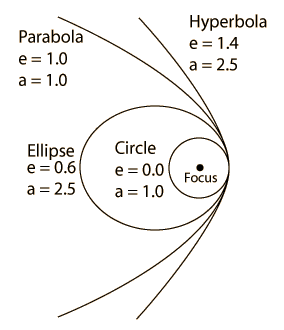
\includegraphics[scale=.65]{./conorb.png}
  \end{figure}
\end{frame}

\begin{frame}
  \frametitle{End of Lesson}
Next Lesson: Vectors.
\end{frame}

\end{document}
